\documentclass{article}
\usepackage[letterpaper, margin=1in]{geometry} % set margins

\usepackage{setspace} % to set spacing
%\singlespacing
\doublespacing

% Figures and colors
\usepackage{graphicx,caption,subcaption} % for figures and captions
\usepackage{xcolor}

% Equations and formulas
\usepackage{amsmath}
\usepackage{amssymb}
\usepackage{bm}
\usepackage{nccmath}
  
% For modelsummary tables
\usepackage{booktabs}
\usepackage{siunitx}

% Codec and language
\usepackage[utf8]{inputenc}
\usepackage[T1]{fontenc}
\usepackage[english]{babel}

% Links and crossreferences
\usepackage{hyperref} % for links
\hypersetup{
    colorlinks,
    linkcolor={red!50!black},
    citecolor={blue!50!black},
    urlcolor={blue!80!black}
}

% References and Appendix
\usepackage[round]{natbib} % for citations


\title{Title\footnote{Note to title}}
\author{First  Author\footnote{Position, Institution Contact: \texttt{\href{mailto:first.last@institution.edu}{first.last@institution.edu}}}
\and
Second  Author\footnote{Position, Institution Contact:  \texttt{\href{mailto:first.last@institution.ed}{first.last@institution.ed}}}}
\date{\today}




\begin{document}
\maketitle

\begin{abstract}
My abstract
\end{abstract}


\newpage
\tableofcontents

\newpage
\section{Introduction}
\label{sec:intro}

\LaTeX is not a WYSIWYG editor like Microsoft Word or Libre Office. Here your text and your formating of the document are separate tasks. 

You write text with formating instructions and \LaTeX will take care of the formating for you. For example, we can decide to make some words \textbf{bold}, \textit{italics}, \underline{underlined}, or \texttt{monospaced}. If you want to link to a source on the internet you can do so with the \texttt{url} or \texttt{href} function. Either like this \url{https://www.wikipedia.com} or like this \href{https://www.wikipedia.com}{Wikipedia}.

In \LaTeX, you don't have to delete text, you can just use the \% symbol to comment text out. It will still be visible in your editor (in a different color) but it won't render in the PDF. This is a super useful tool for writing and editing. Make use of it!
% This text for example, won't be visible in the PDF. 


We can also make numbered lists:

\begin{enumerate}
    \item My first item
    \item My second item
    \item My third item
\end{enumerate} 


We can also make non-numbered lists:


\begin{itemize}
    \item My first item
    \item My second item
    \item My third item
\end{itemize} 

We can also make our own lists. This works great for our hypotehese:


\begin{description}
    \item[H1:] My first item
    \item[H2:] My second item
    \item[H3:] My third item
\end{description} 

\newpage
\section{Theory}
\label{sec:theory}

We can also insert citations! This is an absolutely fanatstic feature of \LaTeX, we can specify the way we want the citation to be added, the information is pulled in from the \texttt{bib} file we specified at the end of the document, and formatted correctly. We also get a nicely formated bibliography!



Hello, this is something someone else said \citep{lee2019machine}.

We can use the following commands:
\begin{enumerate}
    \item \texttt{citep(key1)} \citep{smith2020impact}
    \item \texttt{citet(key1)} \citet{smith2020impact}
    \item \texttt{citeauthor(key1)} \citeauthor{smith2020impact}
    \item \texttt{citeyear(key1)} \citeyear{smith2020impact}
    \item \texttt{citep[text](key1)} \citep[pp.20]{smith2020impact}
    \item \texttt{citep[text][text](key1)} \citep[for example][pp.20]{smith2020impact}
    \item \texttt{citep(key1, key2, key3)} \citep{smith2020impact,brown2018statistics,lee2019machine}
\end{enumerate}


In order for this to work it is important that we have a bib file and correctly specify the path to the bib file at the end of this document. Basically any literature management software produces bib files for you. You can google where your LMS stores the bib file and then change the code at the bottom of the document.


And we can end \texttt{footnotes} into the text easily as well!\footnote{It's really easy!}


We can also insert direct quotes. 

He said, ``Hello'' \citep[p. 10]{smith2020impact}

She replied, ``Hi there!''  \citep[p. 11]{smith2020impact}


Longer quotes can be inserted this way:

\begin{quote}
``Nam liber tempor cum soluta nobis eleifend option congue nihil imperdiet doming id quod mazim placerat facer possim assum. Lorem ipsum dolor sit amet, consectetuer adipiscing elit, sed diam nonummy nibh euismod tincidunt ut laoreet dolore magna aliquam erat volutpat. Ut wisi enim ad minim veniam, quis nostrud exerci tation ullamcorper suscipit lobortis nisl ut aliquip ex ea commodo consequat''\citep[p. 10]{smith2020impact}.
\end{quote}

\newpage
\section{Empirics}
\label{sec:empirics}

\subsection{Methodology}
\label{sec:methods}

While the integration of citations is already absolutely amazing \LaTeX really excels with more complex documents that have math, tables, and figures. For example, below is a small section of a manuscript I am working on. Here you can see how we can effortlessly integrate equations into our text! 


In the individual split-sample regression models, all observations are now conditional on the respective value of $z$: $\mathbb{E}[Y_{i} \mid X, W,Z = 0]  = \alpha_{0} + \alpha_{1}X_{i} + \bm{W \alpha} + \epsilon_{i}$ and $ \mathbb{E}[Y_{i} \mid X, W,Z = 1]  = \gamma_{0} + \gamma_{1}X_{i} + \bm{W\gamma_}  + \epsilon_{i}$. The split-sample models with covariates in this scenario might look very similar to the interactive model with covariates, but they are not. Instead, since all observations are conditional on the value of $z$ in their split the mathematically equivalent interactive model to the new split-sample models is a fully interacted model in which the splitting variable $z$ is interacted with $x$ as well as every $w_j$ in $\bm{W}$: \useshortskip

\begin{equation}
\label{eq:interaction_model_full}
 \mathbb{E}[Y_{i} \mid X,Z]  = \beta_{0} + \beta_{1}X_{i} + \beta_{2}Z_{i}  + \beta_{3} X_{i}Z_{i} + \sum_{j=1}^{k} (\tau_{j} \bm{W}_{j,i} + \delta_{j} \bm{W}_{j,i} Z_{i}) + \epsilon_{i}   
\end{equation}

%where Y is the dependent variable, X is the continuous predictor, Z is the categorical predictor with $z \in \{0,1\}$,  $\bm{W} = w_{1}, w_{2}, ..., w_{k}$ represent the vector of covariates

where $\tau_{j}$ are the coefficients for each covariate, $w_{j}$ when $z = 0$. $\delta_{j}$ are the coefficients for the interaction terms between $z$ and each covariate $w_{j}$, indicating how $w_j$ changes depending on the value of $z$. Each $w_{j}$ has its own coefficient $\tau_{j}$, which represents its effect when $z = 0$. Each interaction term $w_{j} z$ has a coefficient $\delta_j$, which represents the additional effect of $w_{j}$ when $z = 1$.

\subsection{Data}
\label{sec:data}


\newpage
\section{Results}
\label{sec:results}


\subsection{Tables}
\label{sec:tables}

\begin{table}
\centering
\caption{Summary Statistics}
\centering
\begin{tabular}[t]{lrrrrrrr}
\toprule
  & Unique (\#) & Missing (\%) & Mean & SD & Min & Median & Max\\
\midrule
rr\_scale & 18 & 0 & \num{8.5} & \num{4.2} & \num{0.0} & \num{8.0} & \num{16.0}\\
pid7 & 8 & 0 & \num{4.2} & \num{2.3} & \num{1.0} & \num{4.0} & \num{7.0}\\
pk\_index & 5 & 0 & \num{0.4} & \num{0.3} & \num{0.0} & \num{0.5} & \num{1.0}\\
income & 27 & 0 & \num{12.4} & \num{7.5} & \num{1.0} & \num{11.0} & \num{26.0}\\
age & 74 & 0 & \num{48.9} & \num{16.8} & \num{18.0} & \num{49.0} & \num{110.0}\\
educ & 8 & 0 & \num{4.0} & \num{1.7} & \num{1.0} & \num{4.0} & \num{8.0}\\
male & 2 & 0 & \num{0.5} & \num{0.5} & \num{0.0} & \num{0.0} & \num{1.0}\\
knows\_immigrants & 3 & 0 & \num{0.6} & \num{0.5} & \num{0.0} & \num{1.0} & \num{1.0}\\
viol2a & 7 & 0 & \num{4.9} & \num{3.3} & \num{1.0} & \num{8.0} & \num{8.0}\\
selfmon4 & 7 & 0 & \num{5.3} & \num{1.8} & \num{1.0} & \num{5.0} & \num{9.0}\\
\bottomrule
\end{tabular}
\end{table}
    


\begin{table}[htbp]
\centering
\caption{Linear Regression Results \label{tab:ols_rr}}
\centering
\begin{tabular}[t]{lcc}
\toprule
  & Bivariate model & Full model\\
\midrule
(Intercept) & \num{8.914}*** & \num{10.834}***\\
 & (\num{0.120}) & (\num{0.656})\\
Pol. Knowledge & \num{-0.993}*** & \num{-1.321}***\\
 & (\num{0.218}) & (\num{0.206})\\
Asian &  & \num{0.523}\\
 &  & (\num{0.352})\\
Black &  & \num{-2.096}***\\
 &  & (\num{0.228})\\
Hispanic &  & \num{-0.373}\\
 &  & (\num{0.214})\\
Mixed &  & \num{-0.384}\\
 &  & (\num{0.395})\\
Native, PI &  & \num{0.658}\\
 &  & (\num{0.766})\\
PID 7 &  & \num{-0.698}***\\
 &  & (\num{0.030})\\
Income &  & \num{0.010}\\
 &  & (\num{0.010})\\
Age &  & \num{0.041}***\\
 &  & (\num{0.004})\\
Education &  & \num{-0.188}***\\
 &  & (\num{0.044})\\
Male &  & \num{0.229}\\
 &  & (\num{0.135})\\
Knows Immig. &  & \num{-0.743}***\\
 &  & (\num{0.138})\\
Violence justified &  & \num{0.013}\\
 &  & (\num{0.039})\\
Center of attention &  & \num{0.059}\\
 &  & (\num{0.072})\\
\midrule
Num.Obs. & \num{3073} & \num{3061}\\
R2 & \num{0.007} & \num{0.274}\\
\bottomrule
\end{tabular}
\end{table}
    

\newpage
\subsection{Figures}
\label{sec:figures}


Inserting figures is also super easy! We can do it with the \texttt{figure} environment. The code below searches for a pdf in the figures folder and automatically inserts it. We also specify the caption and the label of the figure. Labels allow us to reference to things in our document. We have added section lables so we can reference to Section \ref{sec:figures} or Figure \ref{fig:combined} or Table \ref{tab:ols_rr}. 

% Adding a figure
\begin{figure}[htbp]
    \centering
        \caption{Coefficient Plot for the Models in Table~\ref{tab:ols_rr} Column 1-2}
    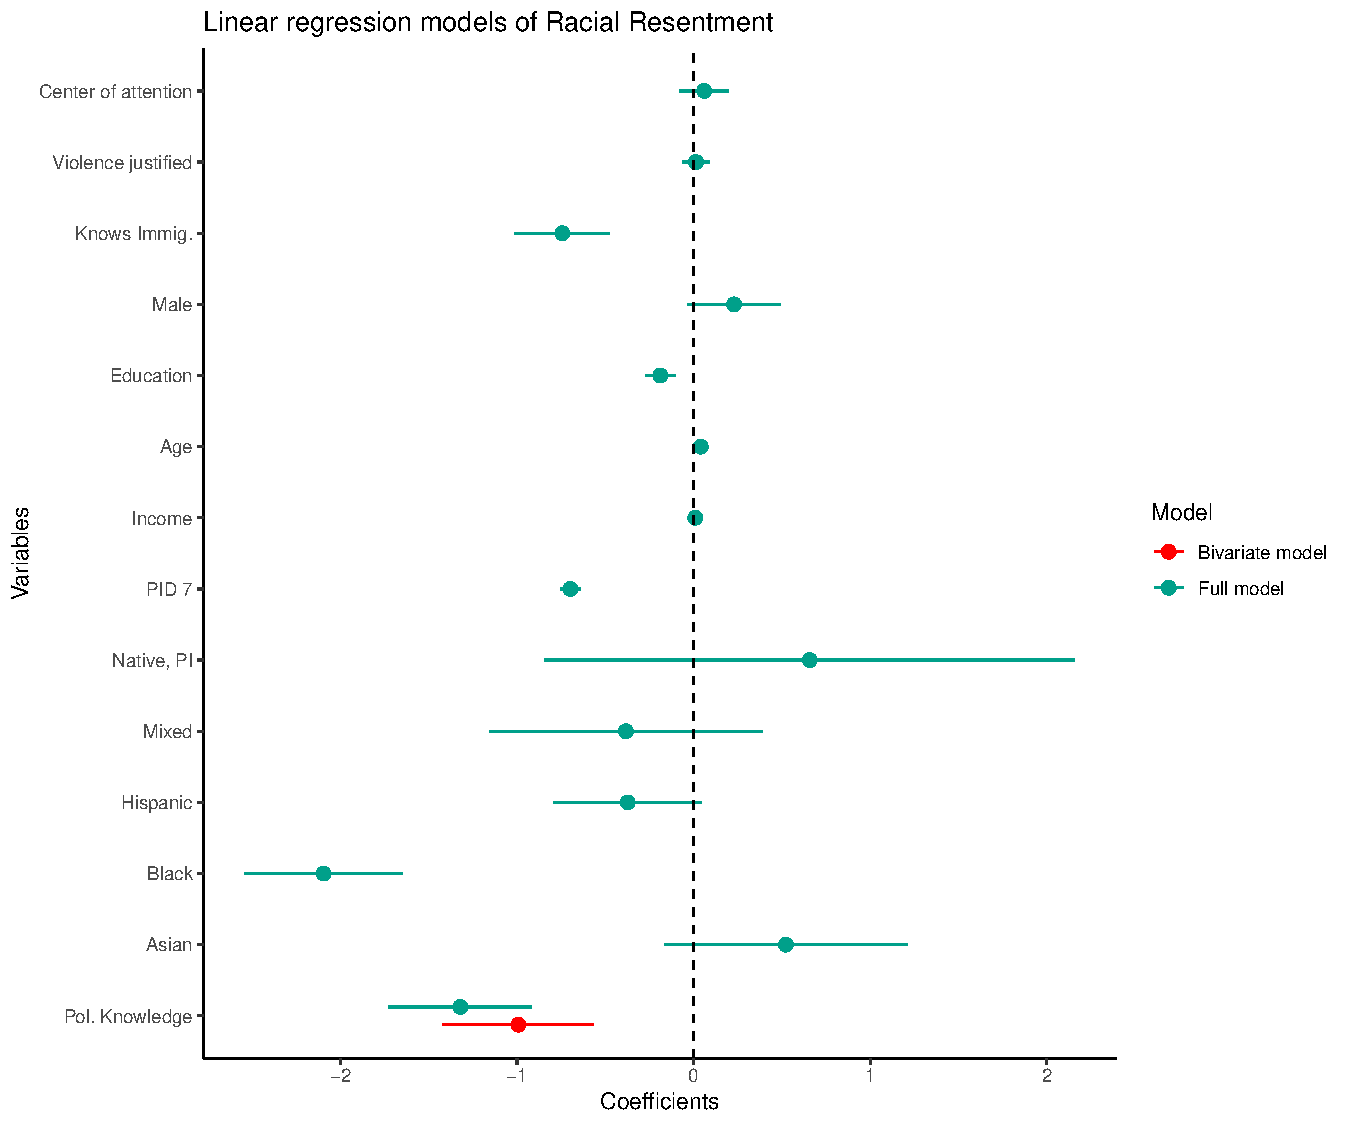
\includegraphics[width=0.8\linewidth]{figures/ols_coefficient_1.pdf}
    \label{fig:ols_coefplot}
\end{figure}


\newpage

We can also display figures next to each other with the \texttt{minipage} environment! In Figure \ref{fig:combined} we can see a bar plot of racial resentment in the ANES Pilot 2020 study in Panel \ref{fig:barplot} and a boxplot of the racial resentment across racialm groups in Panel \ref{fig:boxplot}.

\begin{figure}[htbp] % Placement specifier
\centering
\begin{minipage}{0.48\textwidth} % Adjust width as needed
    \centering
    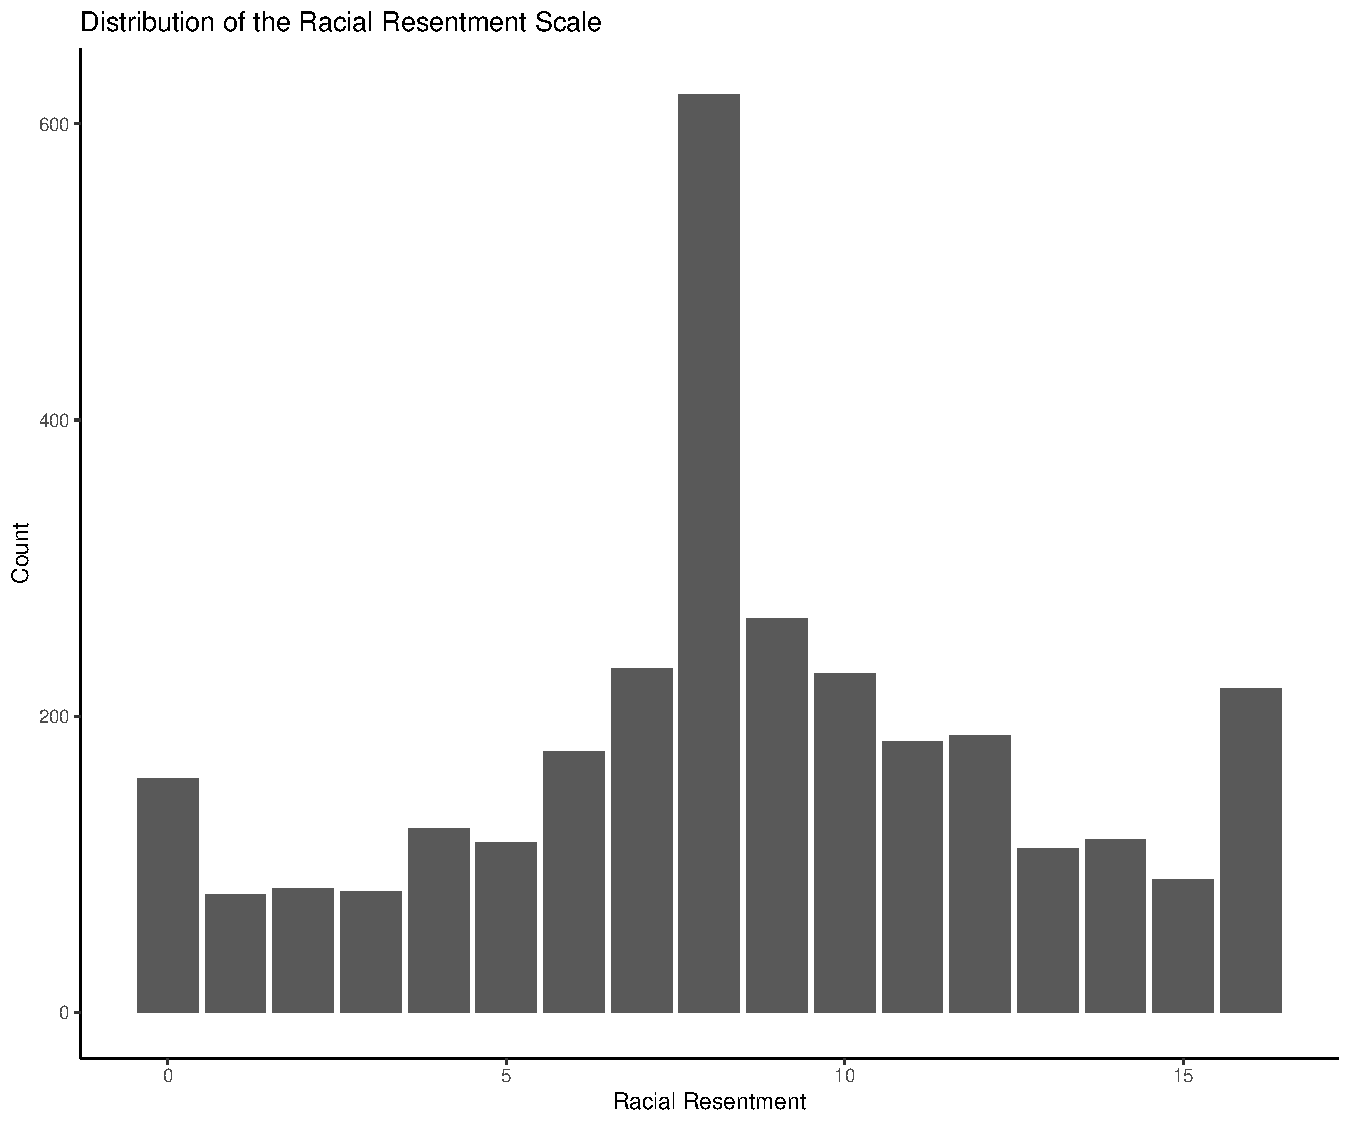
\includegraphics[width=\textwidth]{figures/rr_barplot.pdf} % Path to your first image
        \subcaption{One subfigure}
            \label{fig:barplot}
\end{minipage}
\begin{minipage}{0.48\textwidth} % Adjust width as needed
    \centering
    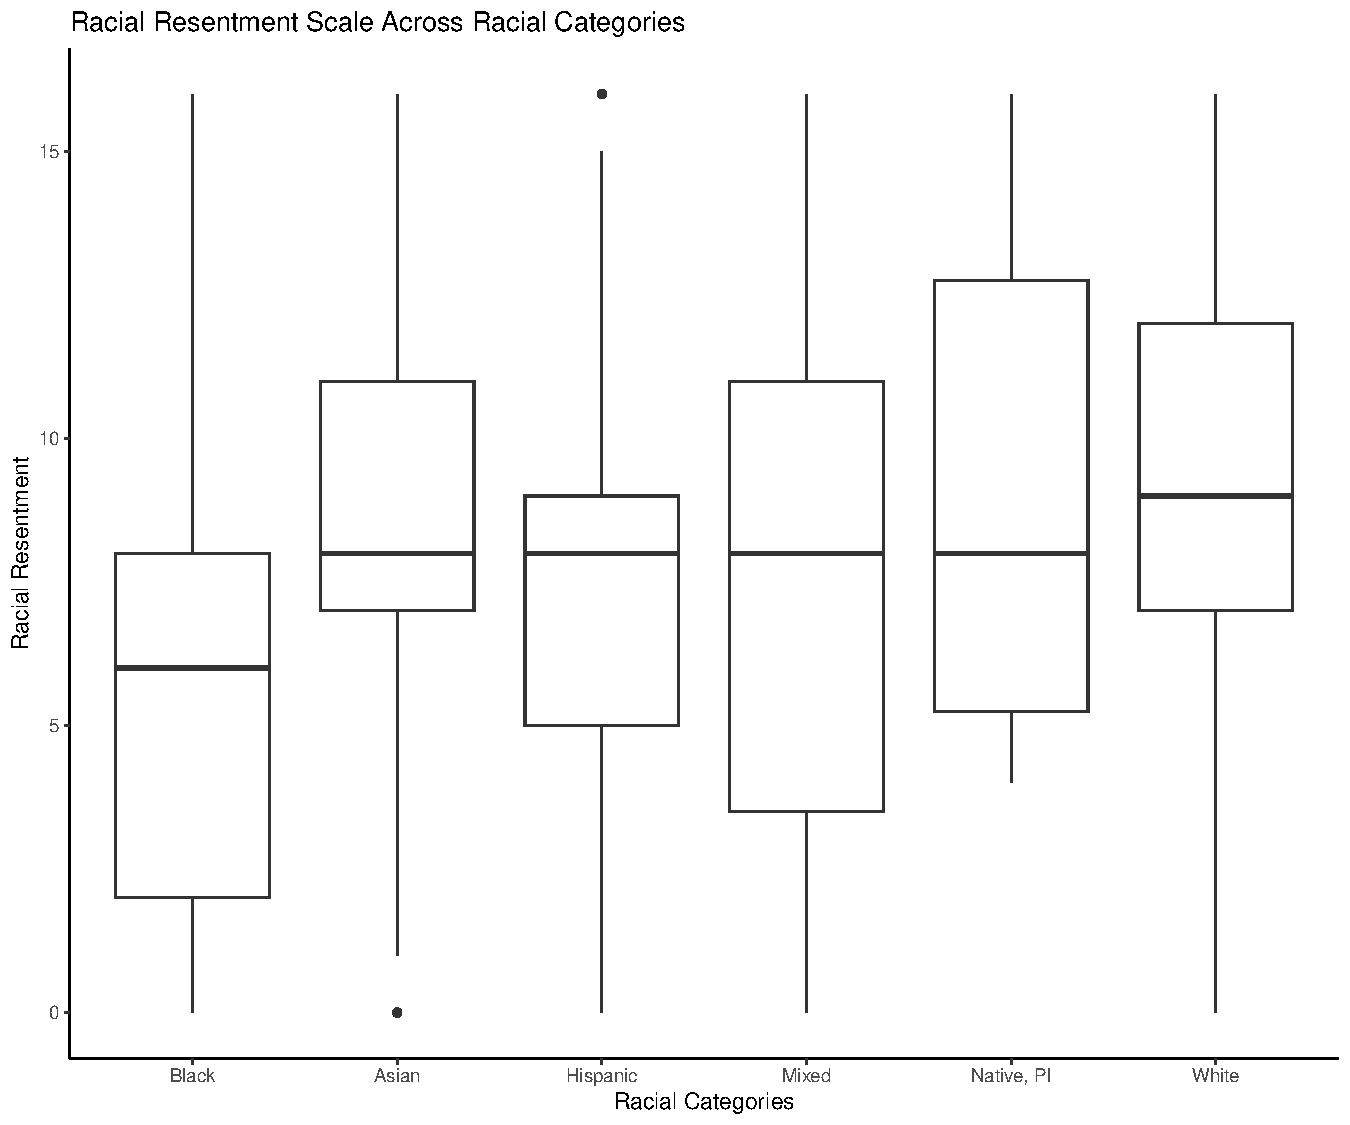
\includegraphics[width=\textwidth]{figures/rr_race_boxplot.pdf} % Path to your second image
    \subcaption{The other subfigure}
    \label{fig:boxplot}
\end{minipage}
\caption{Overlaid Images}
\label{fig:combined}
\end{figure}





\newpage
\section{Discussion}
\label{sec:discussion}

You can also input other \LaTeX documents! This will allow you to write longer documents in spearate parts. I highly recommend you design your Ph.D. dissertation this way. One main document that has your \LaTeX preamble and inputs all your chapters. You don't need to add the preamble or the bibliography information to the individual documents. Just start with a heading and write your chapter. The next chapter is then a different tex file.


\subsection{Text below comes from a different tex document}
\label{sec:imported_section}

Lorem ipsum dolor sit amet, consetetur sadipscing elitr, sed diam nonumy eirmod tempor invidunt ut labore et dolore magna aliquyam erat, sed diam voluptua. At vero eos et accusam et justo duo dolores et ea rebum. Stet clita kasd gubergren, no sea takimata sanctus est Lorem ipsum dolor sit amet. Lorem ipsum dolor sit amet, consetetur sadipscing elitr, sed diam nonumy eirmod tempor invidunt ut labore et dolore magna aliquyam erat, sed diam voluptua. At vero eos et accusam et justo duo dolores et ea rebum. Stet clita kasd gubergren, no sea takimata sanctus est Lorem ipsum dolor sit amet. Lorem ipsum dolor sit amet, consetetur sadipscing elitr, sed diam nonumy eirmod tempor invidunt ut labore et dolore magna aliquyam erat, sed diam voluptua. At vero eos et accusam et justo duo dolores et ea rebum. Stet clita kasd gubergren, no sea takimata sanctus est Lorem ipsum dolor sit amet. 

Duis autem vel eum iriure dolor in hendrerit in vulputate velit esse molestie consequat, vel illum dolore eu feugiat nulla facilisis at vero eros et accumsan et iusto odio dignissim qui blandit praesent luptatum zzril delenit augue duis dolore te feugait nulla facilisi. Lorem ipsum dolor sit amet, consectetuer adipiscing elit, sed diam nonummy nibh euismod tincidunt ut laoreet dolore magna aliquam erat volutpat \citep{garcia2022new,wilson2021climate}. 

Ut wisi enim ad minim veniam, quis nostrud exerci tation ullamcorper suscipit lobortis nisl ut aliquip ex ea commodo consequat. Duis autem vel eum iriure dolor in hendrerit in vulputate velit esse molestie consequat, vel illum dolore eu feugiat nulla facilisis at vero eros et accumsan et iusto odio dignissim qui blandit praesent luptatum zzril delenit augue duis dolore te feugait nulla facilisi \citep{lee2019machine}. 

Nam liber tempor cum soluta nobis eleifend option congue nihil imperdiet doming id quod mazim placerat facer possim assum. Lorem ipsum dolor sit amet, consectetuer adipiscing elit, sed diam nonummy nibh euismod tincidunt ut laoreet dolore magna aliquam erat volutpat. Ut wisi enim ad minim veniam, quis nostrud exerci tation ullamcorper suscipit lobortis nisl ut aliquip ex ea commodo consequat. 




\newpage
\bibliographystyle{apsr}
\bibliography{../resources/bibliography/references.bib}

\end{document}
